\chapter{Fairness}

\qs{}{Che cos'è l'IA?}

\paragraph{Un sistema IA può essere inteso come:}

\begin{itemize}
  \item \fancyglitter{Dati:} esperienza di input presa in considerazione. 
  \item \fancyglitter{Algoritmi:} mezzo per elaborare i dati. 
  \item \fancyglitter{Decisioni:} che possiamo impiegare direttamente o utilizzare come assistenza. 
\end{itemize}

\nt{Per esempio, per Russell e Norvig, il termostato è un esempio di IA.}

\qs{}{Come si può sapere se questo sistema è \fancyglitter{affidabile}?}

\section{Introduzione alla Fairness}

Si può concordare che uno strumento è affidabile se commette un numero limitato di errori, ossia quando è in grado di seguire in modo accurato alle nostre istruzioni. Spesso non è semplice capirlo, esistono due possibili approcci:

\begin{itemize}
  \item \fancyglitter{Metodo Clinico:} il decisore combina o elabora le informazioni nella sua mente. Un metodo IA clinico si basa su una serie di regole prestabilite fornite da un esperto del settore. 
  \item \fancyglitter{Metodo Attuariale o Statistico:} le conclusioni si basano esclusivamente su relazioni empiricamente stabilite tra i dati e la condizione o l'evento di interesse. Un metodo IA attuariale esami i dati passati per prevedere i risultati futuri. 
\end{itemize}

\nt{Grosso modo si sono effettuati metodi clinici dal 1956 al 1990, mentre dal 1980 a oggi si sono sviluppati sistemi attuariali.}

\subsection{Metodo Clinico vs. Metodo Attuariale}

\dfn{Sistemi Esperti}{
  I sistemi esperti hanno rappresentato un'applicazione incredibilmente risucita dell'IA (metodo clinico): se si raccoglie una quantità sufficiente di conoscenze, è possibile costruire una catena di regole che offrono buone prestazioni per un determinato compito.
}

\begin{figure}[h]
    \centering
    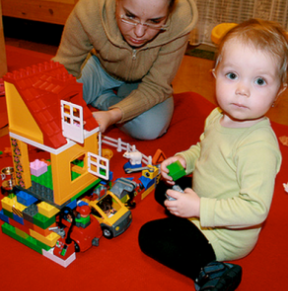
\includegraphics[scale=0.45]{04P/lego.png}
    \caption{Immagine di bambino con mattoncini.}
    \label{fig:mat}
\end{figure}

\qs{}{Cosa si vede nell'immagine \ref{fig:mat}?}

\begin{itemize}
  \item Per anni i ricercatori IA hanno considerato impossibile risolvere questo task con il metodo clinico, ossia definire cosa sia un "bambino" o un "mattoncino" in ogni circostanza. 
  \item Ai giorni nostri è possibile farlo.
  \item Le tecniche di \fancyglitter{apprendimento automatico} (IA attuarie) hanno compiuto progressi teorici e tecnologici. 
  \item Per questo è nata la necessità di sviluppare enormi quantità di dati.
  \item Negli anni dal 2010 in avanti le tecniche di \fancyglitter{deep learning} hanno contribuito a migliorare questo processo.
  \item Le reti neurali hanno maggiore scalabilità rispetto a Hidden Markov Model, Modelli Gaussiani, Reti Bayesiane, etc.
\end{itemize}

\nt{CONTENT WARNING (TW: razzismo, sessismo, autolesionismo, suicidio, ideazione suicida). Saltare a \ref{sec:MLF}.}

\subsection{Esempi del Machine Learing}

\begin{itemize}
  \item Classificazione automatica delle immagini. 
  \item Google Photos tagga due afro-americani come gorilla con il suo software di riconoscimento facciale. 
  \item Un algoritmo IA utilizzato per concorsi di bellezza\footnote{Well i concorsi di bellezza sono intrinsecamente razzisti quindi non era effettivamente un'idea intelligente.}: ai modelli non piacciono le persone di pelle scura.
  \item Modelli di predizione dei crimini: per valutare un "livello di rischio". 
  \item I modelli di scraping AI mostrano una discriminazione nei confronti delle donne\footnote{Che sorpresa...} (fig: \ref{fig:bias}).
    \begin{figure}[h]
    \centering
    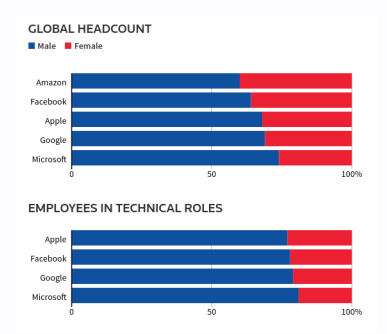
\includegraphics[scale=0.41]{04P/bias.png}
    \caption{Impiegati per sesso (rip NB representation).}
    \label{fig:bias}
\end{figure}
\item I modelli di Amazon avrebbero dovuto essere addestrati a osservare i modelli ricorrenti nei curriculum inviati all'azienda (che erano appunto uomini). 
\item Negli stati uniti le persone con un nome tipicamente bianco hanno più possibilità di essere chiamati per colloqui.
\item Un uomo belga si è suicidato dopo sei settimane di scambi con un chatbot.
\end{itemize}

\qs{}{Ma come è potuto succedere?}

\begin{itemize}
  \item Gli algoritmi sono sessisti/razzisti? 
  \item Chi è il responsabile?
  \item Come hanno fatto gli ingegneri a non notare questi problemi prima dell'implementazione? 
  \item È illegale?
\end{itemize}

\paragraph{Problema:}

\begin{itemize}
  \item L'IA attuariale è spesso \fancyglitter{opaca}: è difficile capire perché un determinato sistema di IA ha preso una particolare decisione. 
  \item Nonostante sia possibile ispezionare i parametri di un modello (il suo algoritmo) collegarli a delle ragioni per cui sono state prese effettivamente delle decisioni. 
\end{itemize}

\section{Machine Learning e Fairness}
\label{sec:MLF}

\dfn{Apprendimento}{
  Si dice che un programma per computer apprende dall'esperienza $E$ rispetto a una classe di compiti $T$ e a una misura di prestazione $P$ se la sua prestazione nei compiti in $T$, misurata da $P$, migliora con l'esperienza $E$.
}

\paragraph{Tasks comuni nel ML:}

\begin{itemize}
  \item \fancyglitter{Classificazione:} dati alcuni dati su entità del mondo reale e un insieme di etichette a essi applicabili, imparare ad assegnare tali etichette a entità non viste. 
  \item \fancyglitter{Regressione:} dati alcuni dati su entità del mondo reale e un insieme di numeri reali a essi applicabili, imparare ad assegnare numeri a entità non viste.
\end{itemize}

\subsection{Classificazione}

\dfn{Classificazione}{
  \begin{itemize}
    \item $X$: dati, covariati. 
    \item $Y$: verità fondamentali, etichette, target variabili.
  \end{itemize}
  La classificazione è il processo che consiste nel determinare un valore plausibile per $Y$ dato $X$. Si cerca di apprendere i parametri $\theta$ di una funzione $f_\theta$ che mappa la variabile casuale $X$ su una stima $\hat Y$ di $Y$:

$$\hat Y = f_\theta (X)$$

}

\cor{Variabile Casuale}{
  Una variabile casuale è un dispositivo matematico utilizzato per descrivere quantità che dipendono da eventi casuali o che sono in generale incerte.
}

\nt{Esempi di variabili casuali: lancio di un dado o di una moneta.}

\begin{figure}[h]
    \centering
    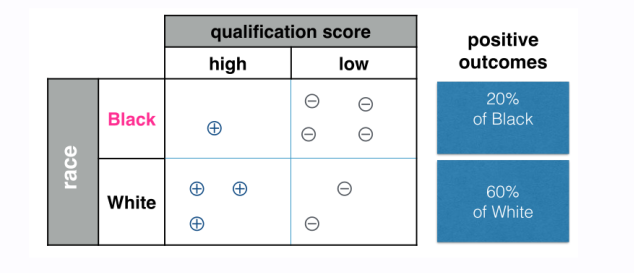
\includegraphics[scale=0.5]{04P/class.png}
    \caption{Esempio di classificazione.}
\end{figure}


\clm{}{}{
  \begin{itemize}
    \item Il processo di apprendimento dei parametri per $f_\theta$ dipende dall'algoritmo e dalla scelta della rappresentazione. 
    \item Per la regressione logistica $\theta$ è un vettore di valori reali la cui lunghezza è uguale $X + 1$ dove $X$ è il numero di colonne. 
    \item La rappresentazione più naturale per $\theta$ può essere diversa se cerchiamo di apprendere un albero decisionale. 
  \end{itemize}
}

\dfn{Accuratezza di un Classificatore}{
  Se $P(Y = f_\theta (X)) = P(Y = \hat Y) = 1$ si ha il classificatore perfetto. In generale $P(Y = \hat Y)$ è l'accuratezza del classificatore.
}

\paragraph{In alcuni casi l'accuratezza potrebbe non essere utile:}

\begin{itemize}
  \item Si vuole prevedere se il prossimo anno si verificherà una pandemia. 
  \item Negli ultimi 2000 anni si sarebbe potuta prevedere una probabilità del 99\% di no. 
  \item Questo mostra che è necessario avere altri modi per descrivere le \fancyglitter{prestazioni del classificatore}.
\end{itemize}

\cor{Costo}{
  Il costo è il numero reale $l(\hat y, y)$ che otteniamo quando classifichiamo un esempio con etichetta $y$ come $\hat y$.
}

\dfn{Classificatore Ottimale}{
Il classificatore ottimale è il classificatore che minimizza 

$$\bbE(l(Y, \hat Y))$$ 

dove $\bbE$ è il valore atteso. 

}

\nt{Due classificatori possono avere la stessa accuratezza ma avere costi differenti.}

\subsection{Il Ciclo ML}

\section{Discriminazione e Misure}


